%% Copernicus Publications Manuscript Preparation Template for LaTeX Submissions
%% ---------------------------------
%% This template should be used for the following class files: copernicus.cls, copernicus2.cls, copernicus_discussions.cls
%% The class files, the Copernicus LaTeX Manual with detailed explanations regarding the comments
%% and some style files are bundled in the Copernicus Latex Package which can be downloaded from the different journal webpages.
%% For further assistance please contact the Publication Production Office (production@copernicus.org).
%% http://publications.copernicus.org


%% Differing commands regarding the specific class files are highlighted.


%% copernicus.cls
\documentclass[ars]{/Users/daviddeboer1/Documents/Papers/Copernicus_LaTeX_Package_v_2_7/copernicus}

%% copernicus2.cls
%\documentclass[journal abbreviation]{/Users/daviddeboer1/Documents/Papers/Copernicus_LaTeX_Package_v_2_7/copernicus2}

%% copernicus_discussions.cls
%\documentclass[ars, hvmath, online]{/Users/daviddeboer1/Documents/Papers/Copernicus_LaTeX_Package_v_2_7/copernicus_discussions}

\def\kperp{k_{\bot}}
\def\kpar{k_{\|}}
\def\nwnh{{\sl NWNH}}

\newcommand{\simgt}{\stackrel{>}{_{\sim}}}
\def\kperp{k_{\bot}}
\def\kpar{k_{\|}}
\def\k{{\bf k}}
\def\sky{{\theta}}
\def\HI{{H{\small I }}}
\def\HII{{H{\small II }}}
\def\xHI{{x_{\rm\HI}}}
\begin{document}

\linenumbers

\title{The Donald C. Backer Hydrogen Epoch of Reionization Array (HERA)}

\author[1]{David R. DeBoer}
\author[2]{James Aguirre}
\author[3]{Judd Bowman}
\author[4]{Richard Bradley}
\author[4]{Chris Carilli}
\author[5]{Josh Dillon}
\author[6]{Steve Furlanetto}
\author[5]{Jacqueline Hewitt}
\author[3]{Daniel Jacobs}
\author[1]{Adrian Liu}
\author[7]{Miguel Morales}
\author[1]{Aaron Parsons}
\author[7]{Jonathan Pober}
\author[5]{Max Tegmark}
\author[1]{Dan Werthimer}

%% each address must have a unique identifier in the option field
\affil[1]{University of California, Berkeley, CA USA}
\affil[2]{University of Pennsylvania, Philadelphia, PA USA}
\affil[3]{Arizona State University, Tempe, AZ USA}
\affil[4]{National Radio Astronomy Observatory, Charlottesville, VA USA}
\affil[5]{Massachusetts Institute of Technology, Cambridge, MA USA}
\affil[6]{University of California, Los Angeles, CA USA}
\affil[7]{University of Washington, Seattle, WA USA}

%% The [] brackets identify the author to the corresponding affiliation, 1, 2, 3, etc. should be inserted.

\runningtitle{HERA}

\runningauthor{DeBoer {\em et al}}

\correspondence{David R. DeBoer\\ (ddeboer@berkeley.edu)}

\received{}
\pubdiscuss{} %% only important for two-stage journals
\revised{}
\accepted{}
\published{}

%% These dates will be inserted by the Publication Production Office during the typesetting process.


\firstpage{1}

\maketitle 

\begin{abstract}
The Donald C. Backer Hydrogen Epoch of Reionization Array (HERA) is a staged
experiment that uses the unique properties of the 21-cm line from neutral
hydrogen to probe the Epoch of Reionization (EoR) and the preceding Dark
Ages. During these epochs, roughly 0.3-1 Gyr after the Big Bang, the first
stars and black holes heat and reionize the Universe following cosmic
recombination. Direct observation of the large scale structure of
reionization and its evolution with time will have
a profound impact on our understanding of the birth of the first galaxies
and black holes, their influence on the intergalactic medium (IGM), and
cosmology.  HERA is a compact hexagonal-packed array of 14-meter paraboloids 
operating from 50 - 225 MHz.
\end{abstract}

\introduction  %% \introduction[modified heading if necessary]
\label{sec:intro}
The Donald C. Backer Hydrogen Epoch of Reionization Array (HERA) is a staged project
that uses the unique properties of the 21-cm line of neutral hydrogen to probe the
Epoch of Reionization (EoR) and the preceding Dark Ages. During these epochs, roughly
0.3-1 Gyr after the Big Bang, the first stars and black holes heated and reionized
the Universe, which at that time existed as a nearly uniform sea of warm neutral
hydrogen.   This period of cosmic reionization represents one of the few global
phase changes in the evolution of the Universe.
Direct observation of the large scale structure of reionization and its
evolution with time will have a profound impact on our understanding of the birth of
the first galaxies and black holes, their influence on the intergalactic medium
(IGM), and cosmology.

Figure \ref{fig:theUniverse} is a cartoon showing cosmic evolution from the Big Bang on the left through
to HERA today.

Detecting, characterizing and ultimately imaging this epoch is a key goal in
furthering our understanding of the Universe and was the top priority in the Radio,
Millimeter, and Sub-millimeter category of recommended new facilities in the most
recent decadal survey of astronomical priorities (\ref{NWNH}). Current projects
(PAPER, MWA, LOFAR, GMRT YYYYYGIVE REFSYYYYY) are striving to make the first detection of the statistical
power spectrum of the signal, but current best limits still fall above even
optimistic predictions of its intrinsic strength. While these projects are still
taking data, it is recognized that an optimized array based on our new understanding
of the signal characteristics is needed to make a strong detection and begin to
characterize this signal over multiple scales and redshifts.

HERA overall is a phased set of experiments that build on its predecessors and preceding stages.
The first phase of the HERA roadmap entailed the operation of the
PAPER and MWA telescopes to explore techniques and designs required to
detect the primordial HI signal in the presence of radio continuum
foreground emission some four orders of magnitude brighter. Studies
with PAPER and the MWA have led to a new understanding of the
interplay of foreground and instrumental systematics in the context of
a three-dimensional cosmological intensity-mapping experiment.  YYYYYGIVE REFSYYYYY 
We are
now able to remove foregrounds to the limits of our sensitivity with
these instruments, culminating in the first physically meaningful
upper limits on the power spectrum of 21~cm emission from
reionization (see Fig \ref{fig:eor_pspec}).

Building on this understanding, the next stage of HERA entails a new
14m diameter antenna element that is optimized both for sensitivity
and for minimizing foreground systematics.  Arranging these elements
in a compact hexagonal grid yields an array that facilitates
calibration, leverages proven foreground removal techniques, and is
scalable to large collecting areas. The array will be located near the current PAPER
experiment
in the radio quiet environment of the SKA site in Karoo, South Africa,
and will have a sensitivity close to two orders of magnitude better than
PAPER and the MWA.  HERA's sensitivity coupled with broader frequency coverage, 
will enable HERA to paint an
uninterrupted picture through reionization, back to the end of the
Dark Ages.  As an array, it can be used in smaller arrays along the way to 
achieve timely science.  Two benchmarks are planned:

HERA~127, deployed in 2016, will measure the rise and fall of the
21~cm reionization power spectrum, constraining the timing and
duration of reionization.

HERA~331, deployed in 2017, will measure fluctuations in the 21~cm
signal over a variety of spatial scales to determine the nature and
distribution of the first galaxies that dominate cosmic
reionization. HERA~331 will also extend precision power-spectrum
observations back to the end of the 'Dark Ages' (z $\sim$ 20), when
the first stars and black holes warm the primordial IGM.

This paper will present a summary of the current understanding
of the signal characteristics and measurements and describe this planned
HERA telescope to be built to detect and characterize the EoR power
spectrum.

\section{Background}
\label{sec:background}
\subsection{Hubble's Law}
\label{sec:hubble}
Modern cosmology has provided a spectacular understanding of the cosmic history of
our Universe starting from the instantaneous moment after the explosion of our
spacetime that we call ``the Big Bang'', which occurred about 13.8 Gyr ago, to the
advent of the large structures that seeded our cosmic current structure. After the
Big Bang, matter and space went streaming outward and is manifest to us by the simple
expression called Hubble's Law:
\begin{equation}
v = H_od
\end{equation}
where $v$ is the velocity of the object away from us, $d$ is the distance to the
object $H_o$ is the so-called ``Hubble Constant'', which has a value of 68 Mpc/km/sec
\ref{planck}, in astronomer's units, where Mpc denotes megaparsecs, where a parsec is
$3.086 \times 10^13$ km. Using measured Doppler shifts one may measure $v$, so if one
knows $H_o$ one may directly compute the distance to the object. Velocity is
typically given as a ``redshift'', denoted as $z$, related to one another by the
non-relativistic Doppler shift equation $z \sim v/c$, where $c$ is the speed of light
in vacuo. And then by Hubble's Law, that redshift conveys a distance.

Note that Hubble's ``Constant'' is a function of time and using $H_o$ denotes today's
value. Determining the evolution of Hubble's constant is essentially the role of
cosmological studies and using Hubble's law for very distant sources requires an
integration with cosmological evolution encoded within it. The values here are
derived from \ref{ned_evo}.

\subsection{Power Spectrum}
\label{sec:pspec}
One tool that is typically employed in studying large scale parameters of the
Universe, is to collapse the richness of its spatial variation to its spatial Fourier
transform and compute a power spectrum of this. It is the parameters of this power
spectrum that may be predicted by cosmology, rather than the essentially random
spatial variation about it. It is analogous to the fact that one may get a few broad
parameters of an FM signal by Fourier transforming its time series, regardless of whether it is
Beethoven or M\"{o}tley Cr\"{u}e, which have very different values as a function of time.

Cosmology typically encodes this data as power in spherical harmonics.  Epoch of
Reionization studies typically use wavevectors, $\k$.  This 3-D vector may be decomposed
into plane-of-sky values (${\bf \kperp}$) and a line-of-sight term (${\kpar}$).  The overall
wavevector may then be written as $\k = {\bf \kperp} + \kpar{\bf z}$.  As a wavevector,
the units of $\k$ are 1/Mpc (inverse length).  Note that although modern cosmology believes
it has pegged the value of Hubble's constant, to hedge their bets, they will often factor out
$h=H_o/100$ as an overall scale adjustment, such that the units are $h$/Mpc.  The units
of the power spectrum magnitudes are given in volume-adjusted power-squared (mK$^2$), denoted
$\Delta ^2$.

\subsection{Foregrounds and Overall Signal Levels}
\label{sec:foregrounds}
At the frequencies of interest (50-250 MHz), the sky as seen by a radio telescope is dominated 
by the synchrotron emission from free electrons spiralling around the magnetic fields that thread
through our Galaxy.  The magnitude of this signal varies as a power law of the frequency, as well
as position on the sky (hottest in the plane of the galaxy, cooler at the poles).  The variation spans
from about 10,000K to about 100K in equivalent temperature.  There are a few localized sources
in the sky that are even hotter to the eyes of a radio telescope.

As will be shown shortly, the signals of interest have equivalent temperatures of $<$ 10 mK, 7 to 9 
orders of magnitude below the foreground signal strengths.  The challenge is to peer through these
strong foreground signals to see the weak signal of interest below.

As stated above, the strong foreground signals may be accurately described as smooth power laws in 
frequency - a factor that may be exploited to extract the signals of interest, which have a structure
that varies fairly rapidly with frequency.

It is also interesting to note that another ``foreground'' from our perspective is the Cosmic Microwave Background.

\section{Scientific Motivation}
\label{sec:science}

The {\it cosmic dawn}, the period beginning with the birth of the first stars and
culminating with the full reionization of the IGM some 500 Myrs later, represents one
of the last unexplored phases in the history of structure formation. During this
period, a wealth of astrophysical and cosmological phenomena are at work. The
characteristics of the IGM depend on the cosmic density field, the formation sites of
the first luminous sources (e.g., their typical masses and clustering), their
constituents (e.g., exotic Population III stars, more normal stars, stellar remnants,
or supermassive black holes) their ultraviolet luminosities (which affect the IGM's
ionization state), the efficiency and abundance of X-ray sources (which affect the
IGM temperature), and even more exotic effects like the relative velocity of baryons
and dark matter.

A season of observing with HERA-127 will yield high-significance constraints on the
21 cm power spectrum across a wide range of k modes and redshifts
\citep{pober_et_al2014}. In Figure \ref{fig:eor_pspec} we show the $z=9$ power
spectrum predicted by the publicly available 21cmFAST software
\citep{mesinger_et_al2011}, along with $2\sigma$ HERA sensitivities. Using the
conservative delay-spectrum (``foreground avoidance") approach pioneered by PAPER
(Parsons et al. 2014), we find that HERA-127 can achieve a $> 10\sigma$ detection of
fiducial power spectra over a broad range of redshifts. The subsequent observing
season with HERA-331 can increase this detection significance to over $25\sigma$
using the same methods. With detailed foreground modeling, the more sophisticated
power spectrum estimator developed for the MWA could increase the size of the ``EoR
window", the region of Fourier space with minimal foreground contamination. This
would allow for an overall detection significance of up to $90\sigma$, along with
access to lower $k$ modes and therefore qualitatively different physics. Such a high
sensitivity measurement would also allow one to go beyond constraining parameters,
testing rather than assuming the underlying theoretical framework and starting to
image the large neutral bubbles during reionization.

%
%\begin{figure}[t]\centering
%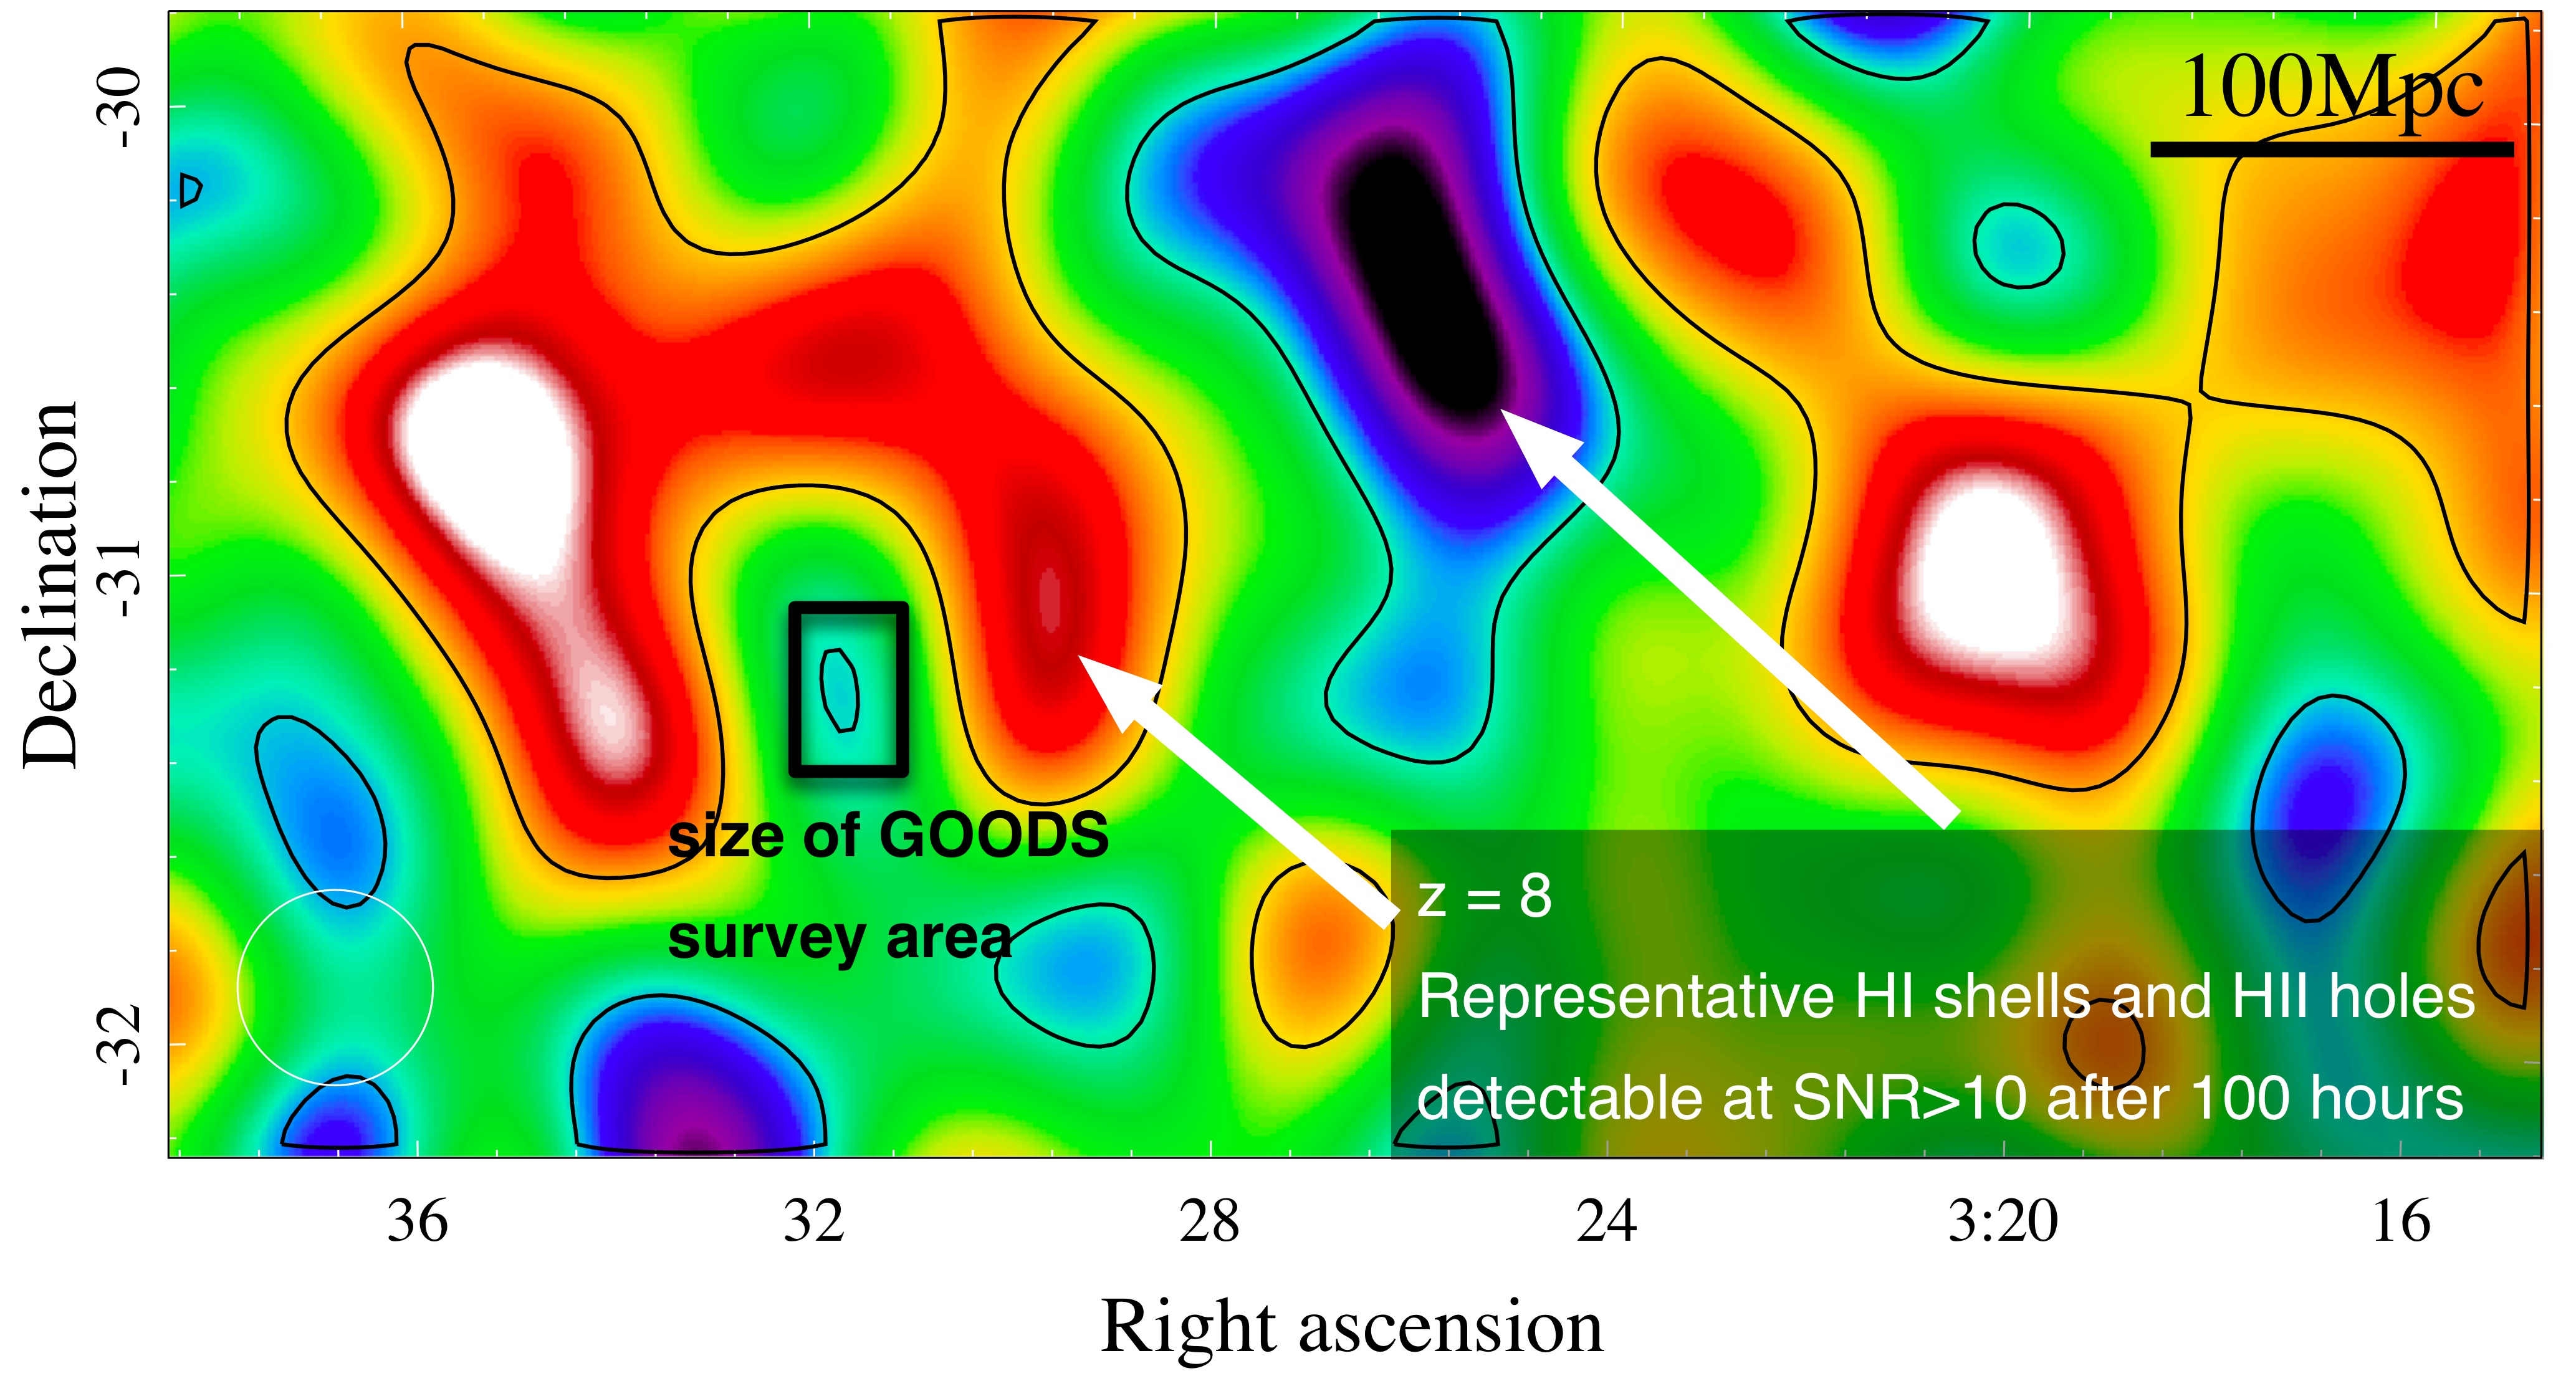
\includegraphics[height=2.5in]{HERA_331_z8_SNR_annotated.jpg}
%\caption{\small
%With sensitivity highly concentrated at the largest scales, 
%HERA-331 will have the sensitivity to directly image HI during reionization.  Shown here is a simulation of EoR emission \citep{mcquinn_et_al2007} as imaged by HERA in 100 hours of observation.  
%Contours enclose regions with signal to noise above 10.  
%With a nearly completely sampled aperture over 300~m across, HERA will have the collecting area of Arecibo but with $500\times$ the survey speed. Each night, HERA drift scans 2600 square degrees.
%}  \label{fig:imaging}
%\end{figure}    

The ability of HERA to image enables an exciting range of cross-correlation science.
HERA HI images reveal the large-scale reionization environment for pointed ALMA and
JWST observations, and other deep near-IR surveys \citep{lidz_et_al2009}. Knowing
whether an observed galaxy is in a region that was previously reionized (center of
large HII bubble), recently reionized (edge of HII bubble), or is forming from
pristine neutral gas provides important contextual information on early galaxy
formation.

The HI images can be cross-correlated with other diffuse tracers of large scale
structure. A number of studies have proposed cross-correlation with large scale
intensity mapping of molecular CO \cite{lidz_et_al2011} and atomic CII
\citep{gong_et_al2011} lines. These studies trace the large scale galaxy distribution
-- the sources of reionization. Prototypes of these experiments may be operating on
the HERA timescale. Such probes have the advantage of having different systematics
compared to HERA, potentially allowing clean measurements of the underlying signal.


VERY SHORT DISCUSSION OF WHAT LIMITS THE EOR BETWEEN Z~12-~6


\section{Specifications}
\label{sec:spec}
The epoch of interest, the spatial scales of interest, the required sensitivity and
the frequency smoothness provide the scientific specifications needed for the array.
Details of the technique, cost, and observing strategies also provide specifications.
This section will discuss these high-level specifications.

\subsection{Frequency Range}
The rest frequency ($\nu_o$) of the hyperfine transition of neutral hydrogen is at
1420.4 MHz. This frequency gets red-shifted to lower frequencies in deep astronomical
observations due to the expansion of the Universe, as discussed above. This is
characterized by the red-shift parameter $z$ as
\begin{equation}
\centering
\label{eq:redshift}
\nu_s(z) = \nu_o/(1+z)
\end{equation}
The age of the Universe at a particular redshift is given by the cosmological model
and a key goal of cosmology is to determine those parameters, however existing models
allow us to determine these values to our desired accuracy. Figure
\ref{fig:theUniverse} plots the red-shifted frequency as a function of red-shift (the
blue curve), with the upper axis showing the cosmic evolution time since the Big Bang
(using parameters from REF PLANCK). The bandwidth for HERA is demarcated by the
horizontal dashed lines. The black dashed lines denote the ``EOR'' core bandwidth,
and the extension to the blue dotted lines is to capture earlier epochs (going lower
in frequency) and find the post-EOR ``null'' (going higher in frequency) as discussed
below. Table \ref{tab:heraband} provides the details of how the frequencies map to
redshift and cosmic time.


\subsection{Bandwidth Field-of-View, and Spatial Scale}
As we've seen above, the frequency at which the hydrogen transition is observed
determines the source's cosmological distance. Therefore the bandwidth of the
observations defines a linear extent along the line-of-sight in space, specified by
the frequencies at the end points. As before, one may compute this extent as a
function of redshift using a cosmological calculator. Note that at large cosmological
distances, relatively narrow bandwidths can imply very large extents, which may have
significant cosmological evolution and hence are effectively different samples of the
Universe. For HERA, this bandwidth limit is about 10 MHz or less. The cosmological
extent for 10 MHz is shown in Figure \ref{fig:heraXY}.

Telescopes have a field-of-view of the observed sky, which gives the two orthogonal
directions to the line-of-sight. A given diameter and redshift will then have a
plane-of-sky extent that with the bandwidth will define a cosmological volume. This
plane-of-sky extent for a 14-meter dish is also shown in \ref{fig:heraXY}.

\subsection{Delay}
To exploit the smooth spectral response filtering of the foregrounds

\subsection{Sensitivity Metric}
The equation for sensitivity has been described in previous works [ref ] and is reproduced below:
\begin{equation}
\centering
\label{eq:sensitivity}
\Delta^2_N(k) 
\end{equation}
Note that $\Delta^2_N(k)$ is the standard radiometric sensitivity equation, scaled by
the volume in $k$-space, normalized by the power spectrum Fourier coefficient, and
reduced by the number of independent samples in a given $k$-mode bin, which may have
both coherent and incoherent application.



Why close-packed.  Hexagonal has 60degree symmetry, not 90degree symmetry like for rectangular.

Why 14-m dishes.

\section{System Overview}
\subsection{Antenna}
14-m

\subsection{Analog System}
amplifiers and stuff

\subsection{Digital System}
fpga and gpus and stuff

\section{Site}
Karoo


\conclusions  %% \conclusions[modified heading if necessary]
And sugar and spice




%\appendix
%\section{\\ \\ \hspace*{-7mm} HEADING}    %% Appendix A
%And everything nice.
%\subsection                               %% Appendix A1, A2, etc.
%And everything else.



\begin{acknowledgements}
TEXT
\end{acknowledgements}




\begin{thebibliography}{}

\bibitem[AUTHOR(YEAR)]{LABEL}
REFERENCE 1

\bibitem[AUTHOR(YEAR)]{LABEL}
REFERENCE 2

...

\end{thebibliography}


%% Literature citations
%% command                        & example result
%% \citet{jones90}|               & Jones et al.\ (1990)
%% \citep{jones90}|               & (Jones et al., 1990)
%% \citep{jones90,jones93}|       & (Jones et al., 1990, 1993)
%% \citep[p.~32]{jones90}|        & (Jones et al., 1990, p.~32)
%% \citep[e.g.,][]{jones90}|      & (e.g., Jones et al., 1990)
%% \citep[e.g.,][p.~32]{jones90}| & (e.g., Jones et al., 1990, p.~32)
%% \citeauthor{jones90}|          & Jones et al.
%% \citeyear{jones90}|            & 1990

%% FIGURES %%%%%%%%%%%%%%%%%%%%%%%%%%%%%%%%%%%%%%%%%%%%%%%%%%%%%%%%%%%%%%%%%%%%

\begin{figure*}[ht]
\vspace*{2mm}
\begin{center}
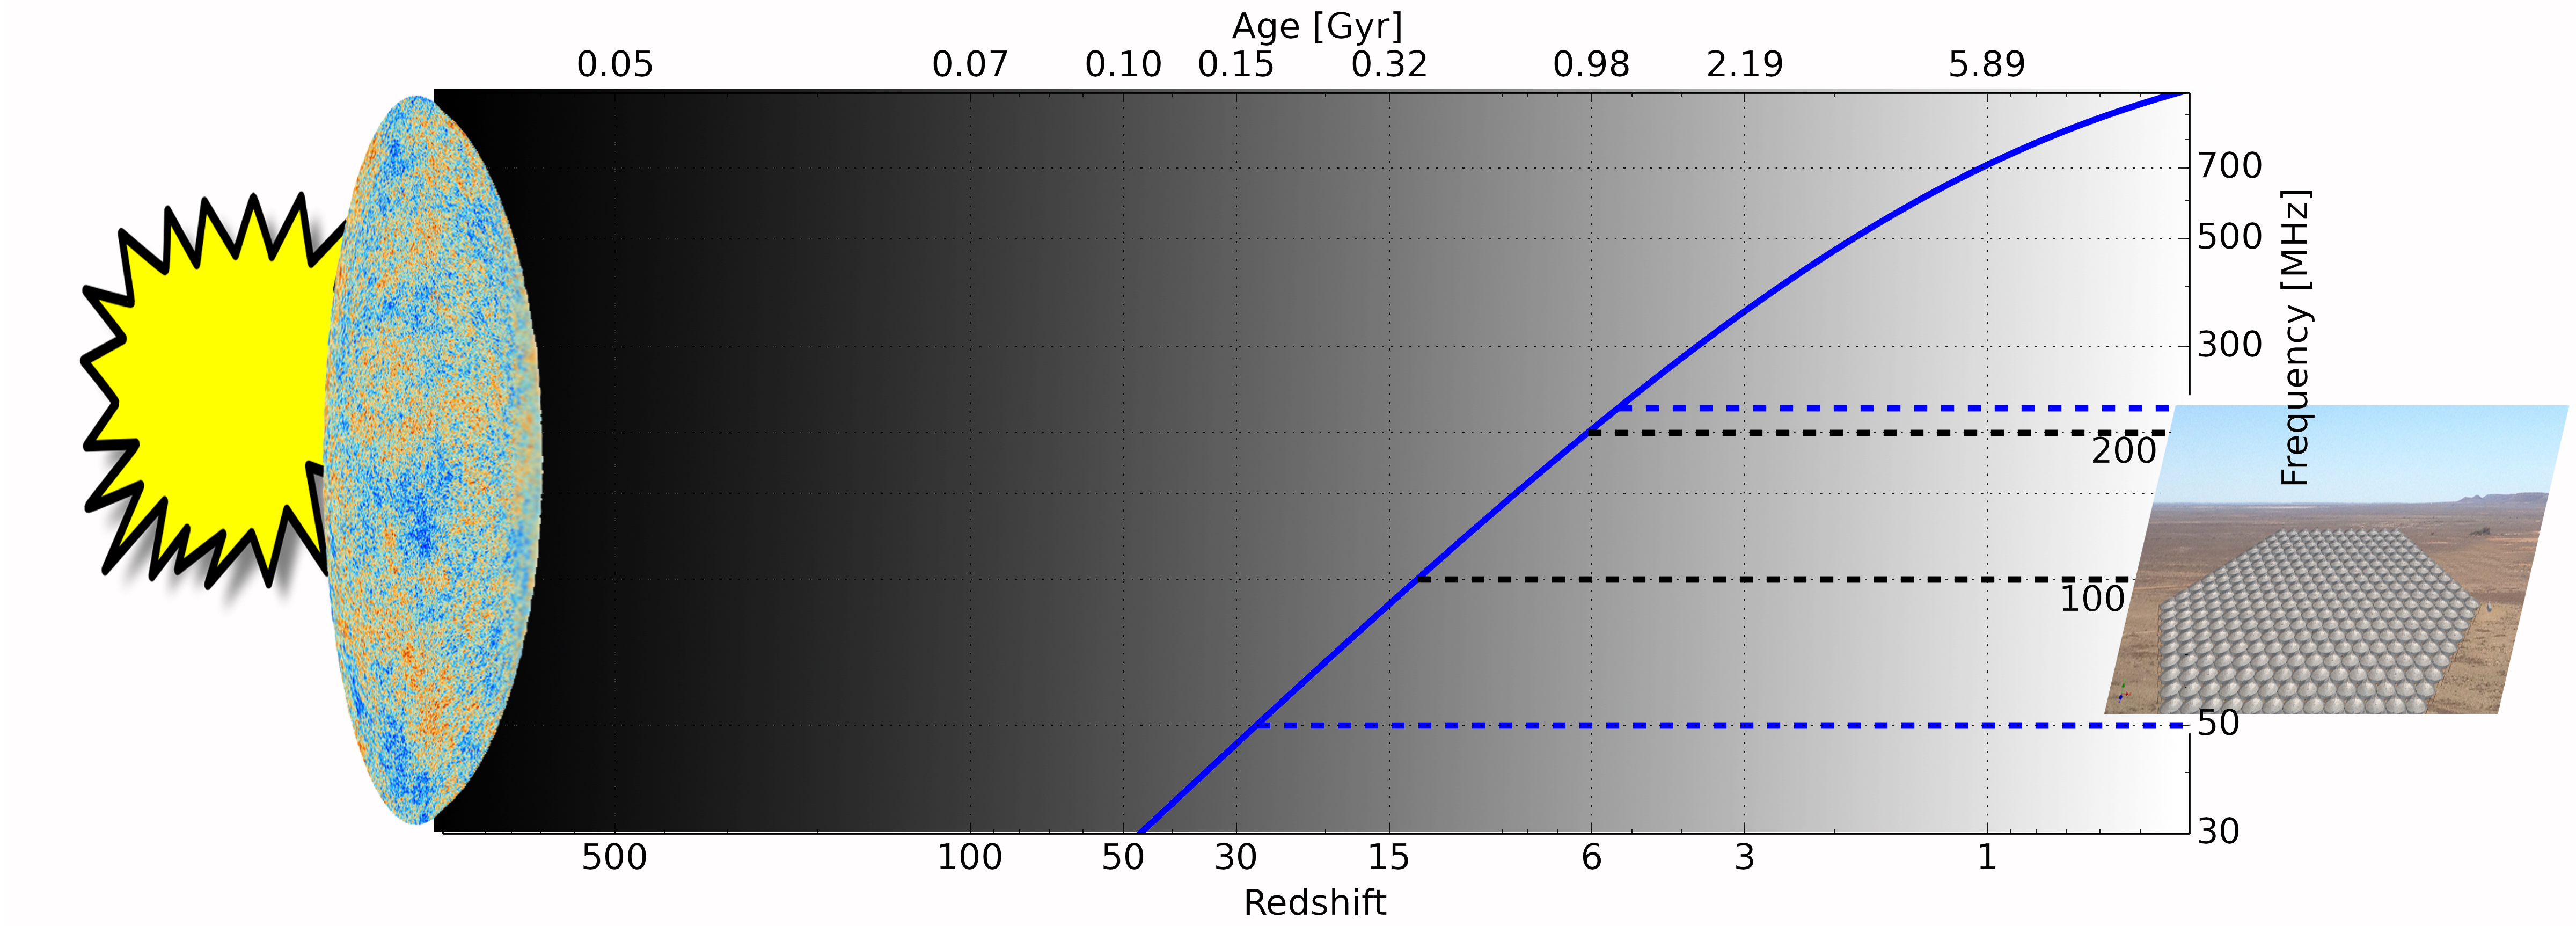
\includegraphics[width=\textwidth]{plots/herauniall.png}
\end{center}
\caption{\small Cartoon showing the development of the Universe and HERA's observing window into it (dashed lines).  The blue solid
line shows the \HI transition frequency as a function of redshift/cosmic evolution age.  The black dashed lines indicate the HERA EOR ``core'' band and blue dashed lines the expanded band, which are detailed in Table \ref{tab:heraband}.}
\label{fig:theUniverse}
\end{figure*}


\begin{figure}[t]\centering
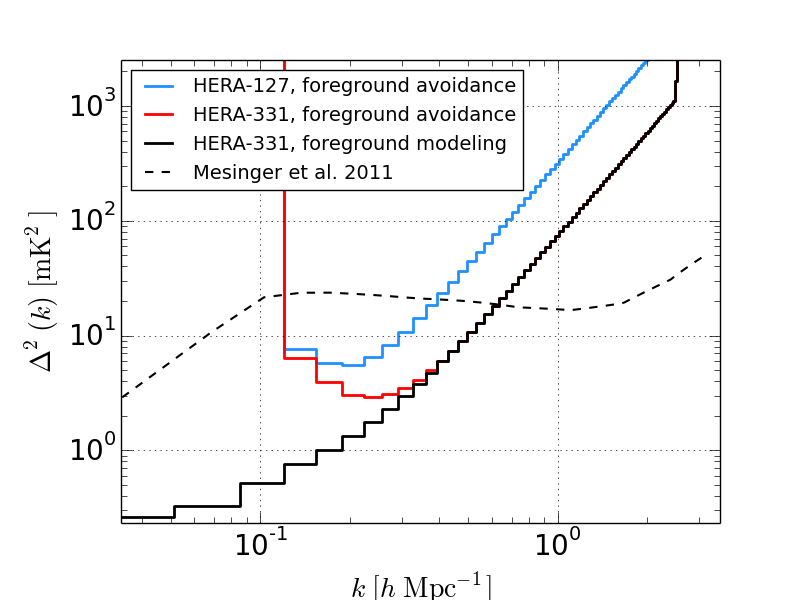
\includegraphics[width=\columnwidth]{plots/eor_pspec_2014.png}
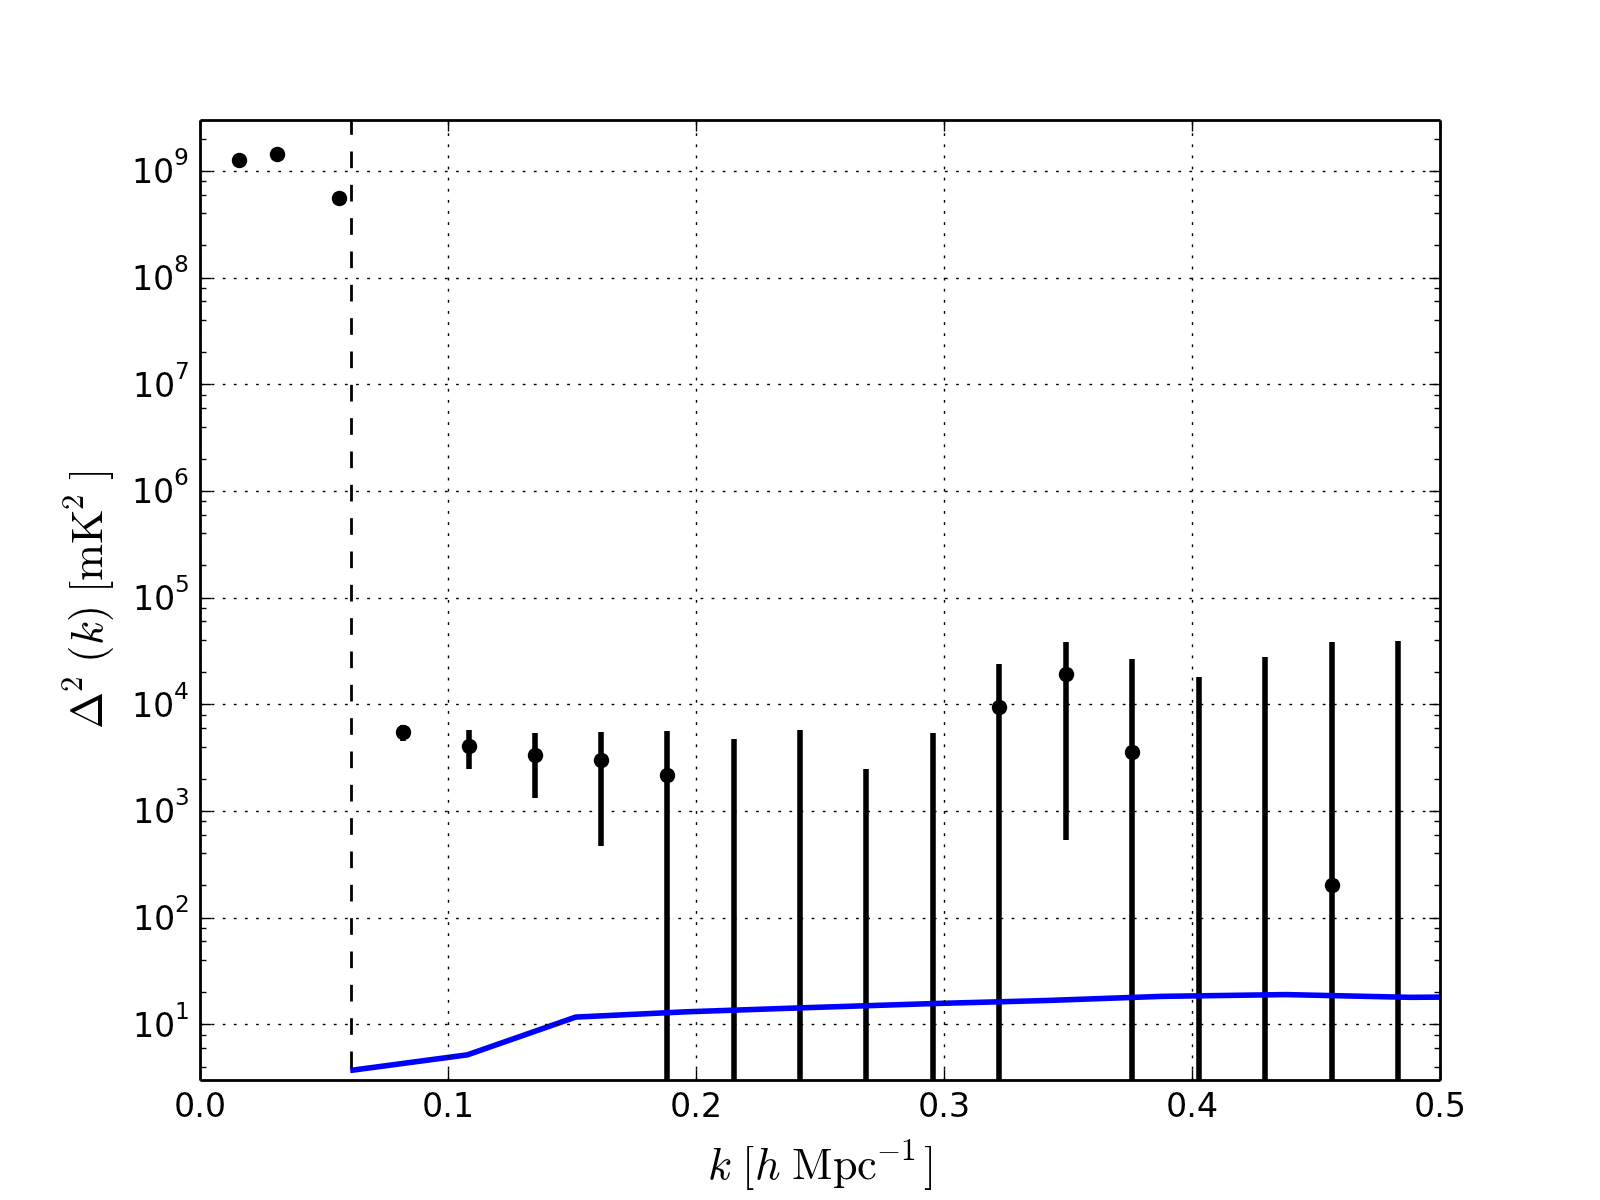
\includegraphics[width=\columnwidth]{plots/hera_pk3pk.png}
\caption{\small Top: HERA's power-spectrum sensitivity (solid)
relative to a fiducial ionization model (dotted line; $\xHI=0.37$, $z=9.0$).  
Sensitivities reflect staged array size and
improving analysis software that expands the range
of modes free of foreground systematics. 
Bottom: The current best upper limit on the 21~cm reionization power spectrum,
obtained with a 32-element PAPER deployment \citep{parsons_et_al2013}.  These upper limits
constrain the brightness temperature of the IGM at $z\sim8$, showing
a departure from adiabatic cooling presumed to be indicative of X-ray heating.
}\label{fig:eor_pspec}
\end{figure}

\begin{figure}[t]
\vspace*{2mm}
\begin{center}
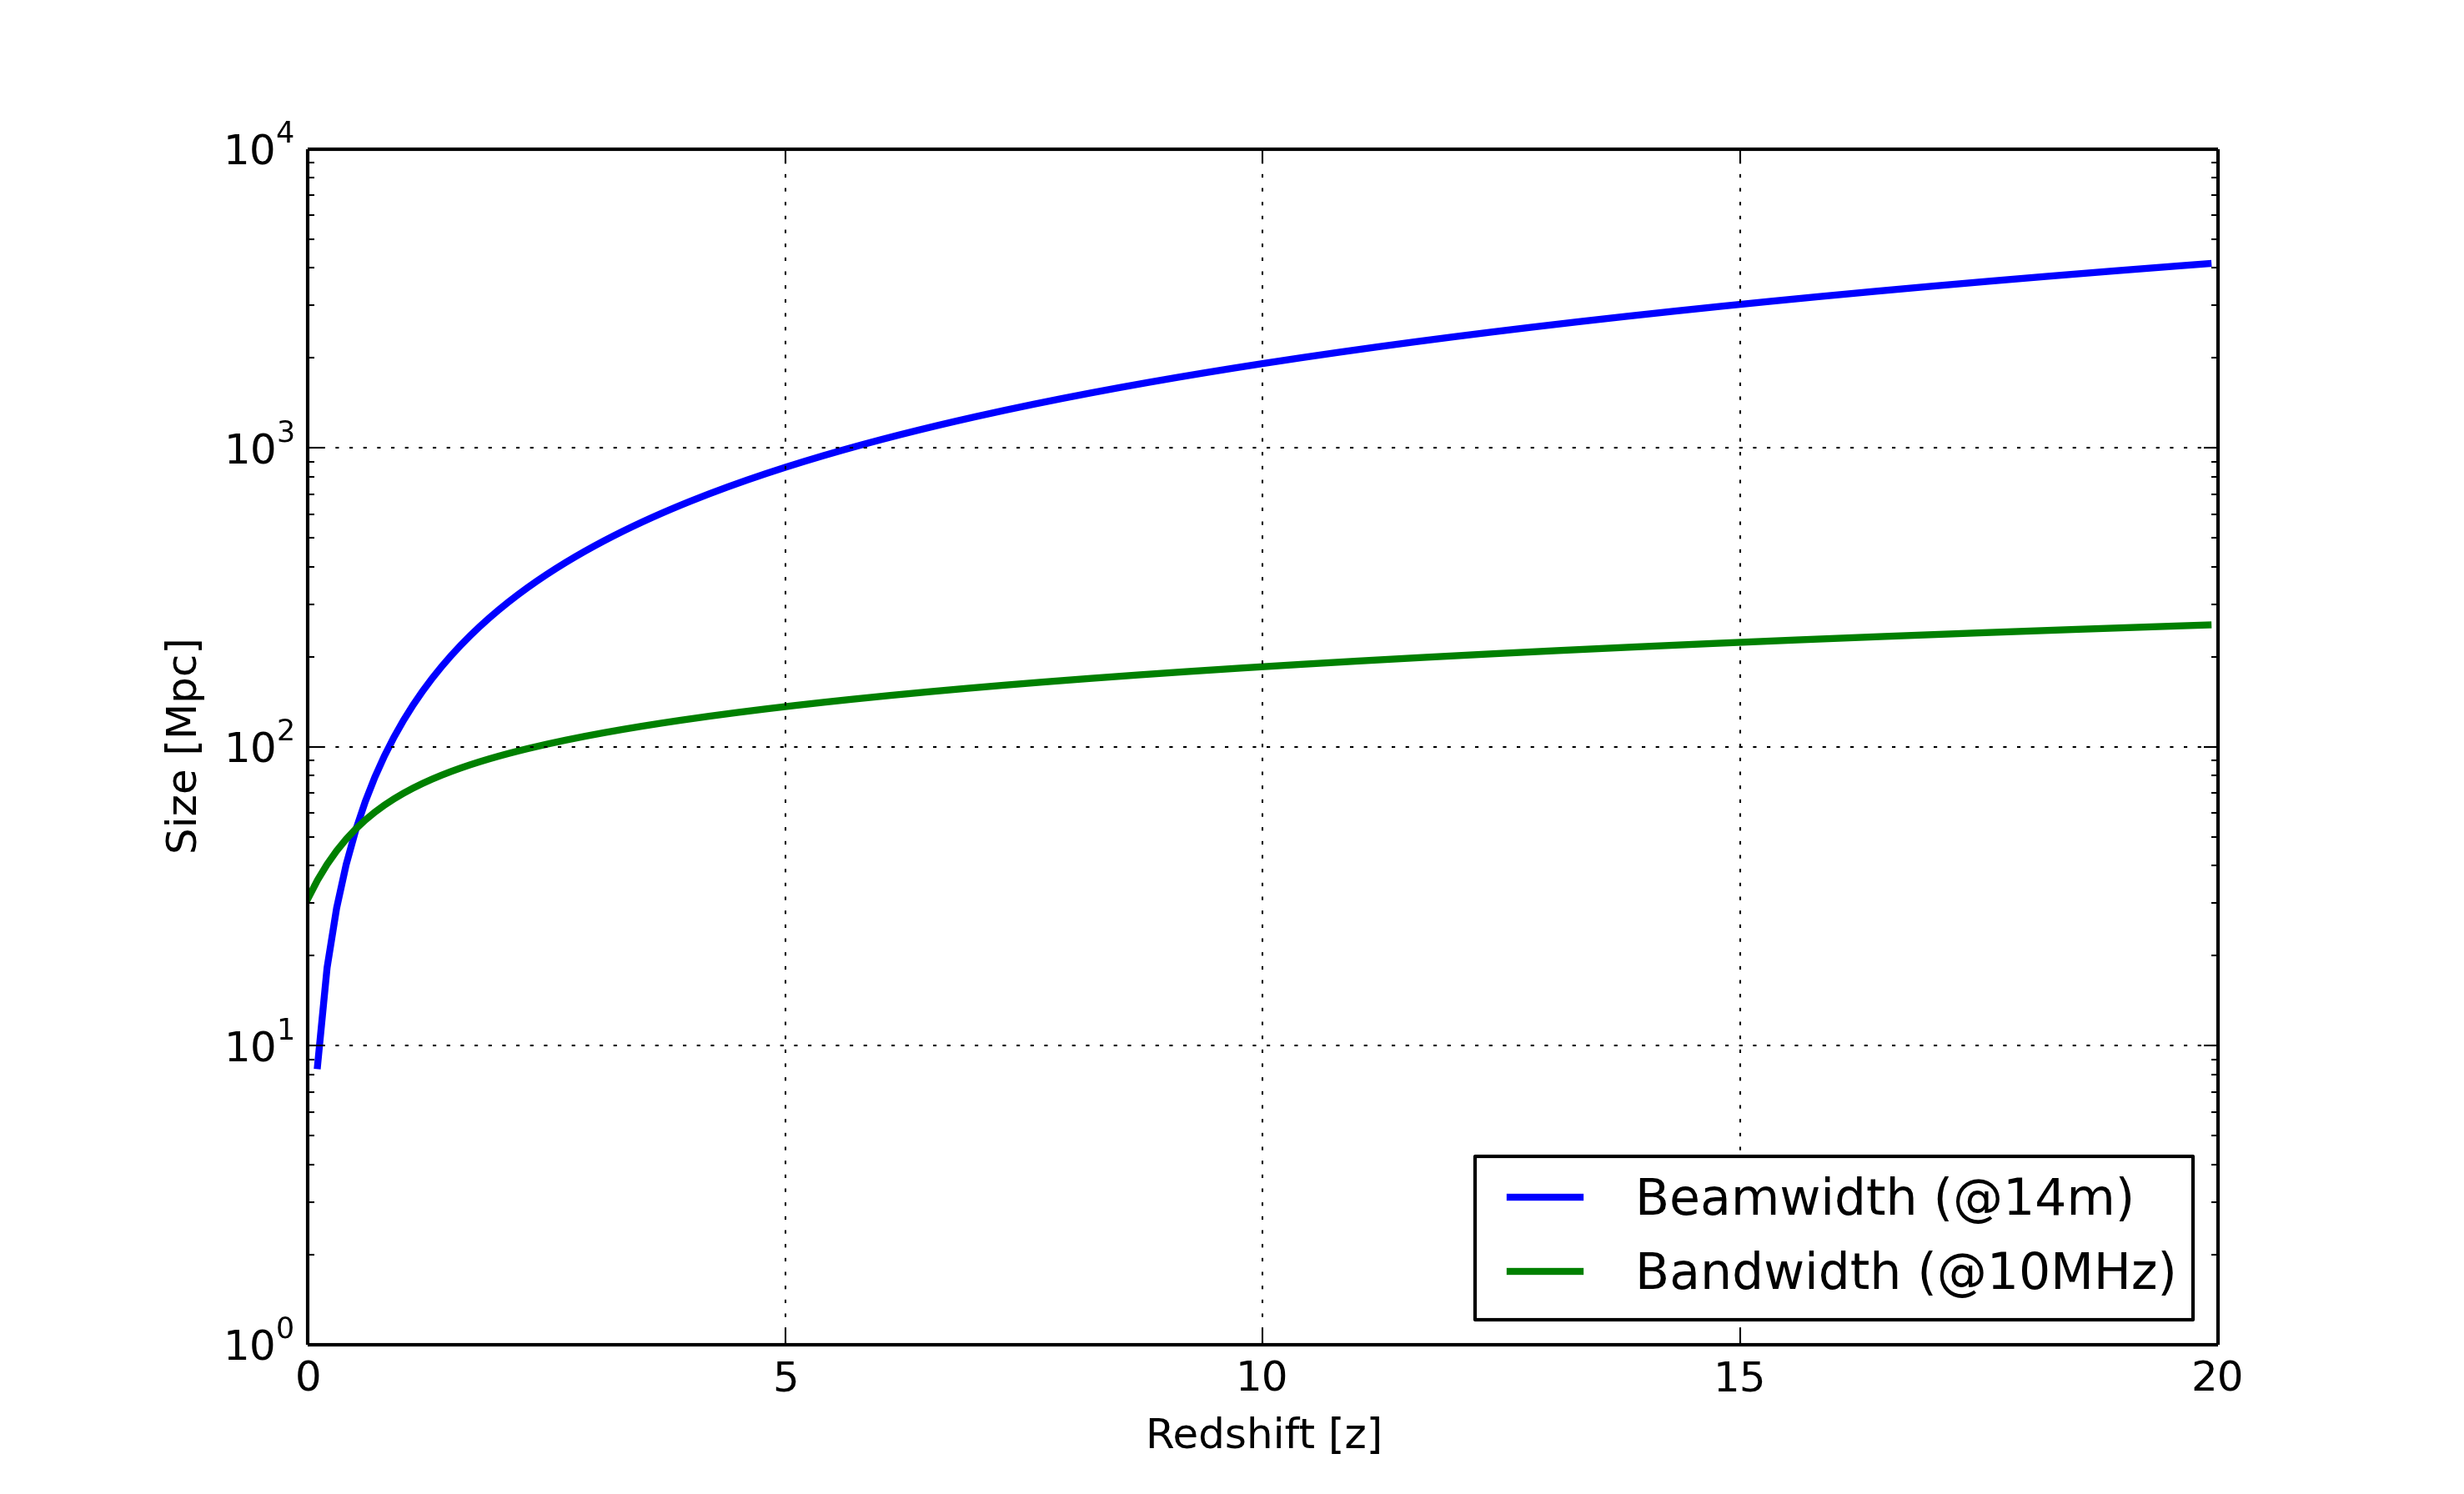
\includegraphics[width=\columnwidth]{plots/heraXY.png}
\end{center}
\caption{Scaling  \label{fig:heraXY}}
\end{figure}


%% TWO-COLUMN FIGURES

%f
%\begin{figure*}[t]
%\vspace*{2mm}
%\begin{center}
%\includegraphics[width=12cm]{FILE NAME}
%\end{center}
%\caption{TEXT}
%\end{figure*}


%% TABLES %%%%%%%%%%%%%%%%%%%%%%%%%%%%%%%%%%%%%%%%%%%%%%%%%%%%%%%%%%%%%%%%%%%%
\begin{table*}[t]
\caption{HERA band in frequency, redshift, cosmic age and comoving distance.}
\label{tab:heraband}
\vskip4mm
\centering
\begin{tabular}{| c | c | c | c |} \hline
\textbf{Frequency [MHz]} & \textbf{Redshift} & \textbf{Age} & \textbf{Look-back} \\
\textbf{[MHz]}                   &                            & \textbf{[Myr]}  & \textbf{[Gly]} \\ \hline
50 & 27.4    & 164 & 13.6 \\ \hline
100 & 13.2  & 372 & 13.4 \\ \hline
200  & 6.1    & 960  & 12.8 \\ \hline
225  &  5.3   & 1,135  &  12.7 \\ \hline
\end{tabular}
\end{table*}



%% ONE-COLUMN TABLE

%t
%\begin{table}[t]
%\caption{TEXT}
%\vskip4mm
%\centering
%\begin{tabular}{column = lcr}
%\tophline

%\middlehline

%\bottomhline
%\end{tabular}
%\end{table}


%% TWO-COLUMN TABLE

%t
%\begin{table*}[t]
%\caption{TEXT}
%\vskip4mm
%\centering
%\begin{tabular}{column = lcr}
%\tophline

%\middlehline

%\bottomhline
%\end{tabular}
%\end{table*}


%% The different columns must be seperated with a & command and should
%% end with \\ to identify the column brake.

%%%%%%%%%%%%%%%%%%%%%%%%%%%%%%%%%%%%%%%%%%%%%%%%%%%%%%%%%%%%%%%%%%%%%%%%%%%%%%


%% If figures and tables must be numbered 1a, 1b, etc. the following command
%% should be inserted before the begin{} command.

%\addtocounter{figure}{-1}\renewcommand{\thefigure}{\arabic{figure}a}


\end{document}
